\sectioncounter{9}
  \section{对数函数}

  \subsection{知识梳理}
  形如 $y=\log_a x$ 的函数称为\myindex{对数函数} (logarithmic function), 其中 $0<a<1$ 或 $a>1$. 分别考虑对数函数 
  $y= \log_2 x$ (如图~\ref{fig-190216-1640}) 和 $y=\log_{\frac12} x$ 
  (如图~\ref{fig-190216-1645}) 的图像可以知道, 对数函数 $y=\log_a x$ 恒过点~$(1,0)$, 
  并以 $x=0$ 即 $y$~轴为渐近线, 且当 $0<a<1$ 时单调递减, 而当 $a>1$ 时单调递增.
  
  \mymarginpar{对下图中的四个对数函数图象, 借助 $y=1$ 可知 $0<c<d<1<a<b$.
    \begin{center}
    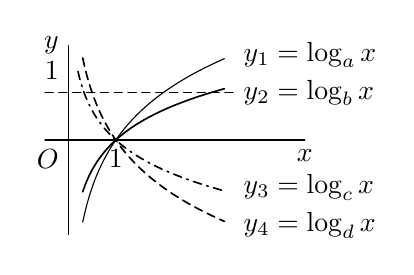
\begin{tikzpicture}[line cap=round,line join=round,scale=0.6]
      \draw[\myaxisarrow] (-0.5,0) -- (5,0) node[below] {$x$};
      \draw[\myaxisarrow] (0,-2) -- (0,2) node[left] {$y$};
      \draw[line width=0.6pt,smooth,samples=100] 
        plot[domain=0.3:3.3](\x,{ln(\x)/ln(3)});
      \draw[line width=0.4pt,smooth,samples=100] 
        plot[domain=0.3:3.3](\x,{ln(\x)/ln(2)});
      \draw[line width=0.6pt,smooth,samples=100,densely dashed] 
        plot[domain=0.3:3.3](\x,{ln(\x)/ln(0.5)});
      \draw[line width=0.6pt,smooth,samples=100,dash dot] 
        plot[domain=0.2:3.3](\x,{ln(\x)/ln(0.33)});
      \draw[densely dashed] (-0.5,1)--(3.5,1);
      \draw (0,0) node[anchor=north east] {$O$}
        (1,0) node[below] {$1$} 
        (0,1) node[left,yshift=8pt] {$1$}
        (3.5,1.8) node[right] {$y_1=\log_a x$} 
        (3.5,1) node[right] {$y_2=\log_b x$}
        (3.5,-1) node[right] {$y_3=\log_c x$} 
        (3.5,-1.8) node[right] {$y_4=\log_d x$};
    \end{tikzpicture}\end{center}}
    
  \begin{figure}[htb]
  \small\centering
  \begin{minipage}[b]{0.4\linewidth}
  \centering
  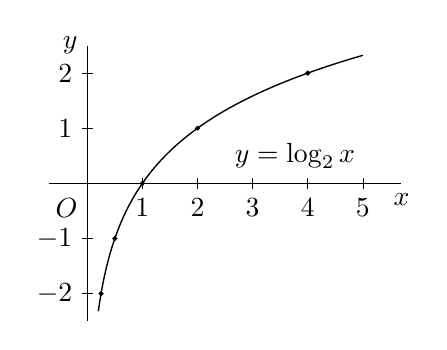
\begin{tikzpicture}[scale=0.7]
    \draw[\myaxisarrow] (-0.7,0)--(5.7,0) node[below] {$x$};
    \draw[\myaxisarrow] (0,-2.5)--(0,2.5) node[left] {$y$};
    \draw (2.5,0.5) node[right] {$y=\log_2 x$};
    \draw[line width=0.5pt,smooth,samples=100,domain=0.2:5] plot(\x,{ln(\x)/ln(2)});
    \foreach \x in {1,2,...,5}
      {\draw[line width=0.2pt] (\x,-0.1) node[below] {$\x$} --(\x,0.1);}
    \foreach \y in {-2,-1,1,2}
      {\draw[line width=0.2pt] (-0.1,\y) node[left] {$\y$}--(0.1,\y);}
    \draw (0,-0.1) node[anchor=north east] {$O$};
    \draw [fill=black] (1,0) circle (1pt) (0.5,-1) circle (1pt)
      (0.25,-2) circle (1pt) (2,1) circle (1pt)
      (4,2) circle (1pt);
  \end{tikzpicture}
  \caption{}\label{fig-190216-1640}
  \end{minipage}
  \hskip 1cm%
  \begin{minipage}[b]{0.4\linewidth}
  \centering
  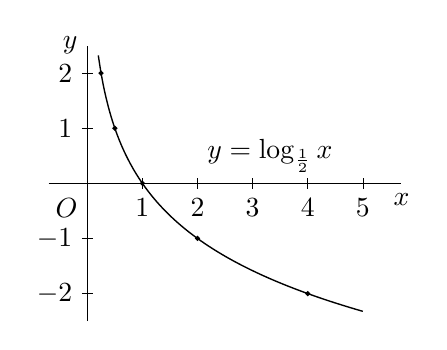
\begin{tikzpicture}[scale=0.7]
    \draw[\myaxisarrow] (-0.7,0)--(5.7,0) node[below] {$x$};
    \draw[\myaxisarrow] (0,-2.5)--(0,2.5) node[left] {$y$};
    \draw (2,0.5) node[right] {$y=\log_{\frac12} x$};
    \draw[line width=0.5pt,smooth,samples=100,domain=0.2:5] plot(\x,{-ln(\x)/ln(2)});
    \foreach \x in {1,2,...,5}
      {\draw[line width=0.2pt] (\x,-0.1) node[below] {$\x$} --(\x,0.1);}
    \foreach \y in {-2,-1,1,2}
      {\draw[line width=0.2pt] (-0.1,\y) node[left] {$\y$}--(0.1,\y);}
    \draw (0,-0.1) node[anchor=north east] {$O$};
    \draw [fill=black] (1,0) circle (1pt) (0.5,1) circle (1pt)
      (0.25,2) circle (1pt) (2,-1) circle (1pt)
      (4,-2) circle (1pt);
  \end{tikzpicture}
  \caption{}\label{fig-190216-1645}
  \end{minipage}
  \end{figure}
  
  对数函数的单调性常用来估计指数式的值, 进而比较对数式之间或对数式与其它式子 
  (如指数式) 的大小. 例如, 考虑 $\log_2{0.6}$ 和 $\log_{0.5}0.6$, 因为
  \begin{align*}
    \log_2{0.5}<\log_2{0.6}<\log_2{1} &\text{\ 即\ } -1<\log_2{0.6}<0,\\ 
    \log_{0.5}1<\log_{0.5}0.6<\log_{0.5}0.5 &\text{\ 即\ } 0<\log_{0.5}0.6<1,
  \end{align*}
  所以 $\log_2{0.6}<\log_{0.5}0.6$. 大部分对数式比较大小的问题, 一般只要考虑与 $0$, $1$ 
  的大小关系即可得到答案. 比如在前面的问题中, 因为 $\log_2{0.6}<0<\log_{0.5}0.6<1$, 
  自然有 $\log_2{0.6}<\log_{0.5}0.6$.

  \lianxi
  \begin{exercise}
    函数 $y=\ln(x^2 -1)$ 的定义域为\,?
  \end{exercise}

  \beginsolution
    由 $x^2-1>0$ 知 $x\in(-\infty,-1)\cup (1,+\infty)$.
  \endsolution
  
  \begin{exercise}
    函数 $f(x)=\log_a (x-1)$ 的图象经过的定点是\,?
  \end{exercise}

  \beginsolution
    由 $\log_a 1=0$ 知 $f(2)=0$, 即 $f(x)$ 的图象过定点 $(2,0)$.
    
    \varexercise 函数 $f(x)=\log_a (x^2-3)+x$ 的图象经过的定点是\,?
    
    由 $\log_a 1=0$ 知 $f(\pm2)=\pm2$, 即 $f(x)$ 的图象过定点 $(-2,-2)$ 和 $(2,2)$.
  \endsolution
  
  \begin{exercise}
    已知 $a=3^{0.2}$, $b=0.3^2$, $c=\log_{0.3}2$, 
    那么 $a$, $b$, $c$ 的大小关系为\,?
  \end{exercise}

  \beginsolution
    $c<0<b<1<a$, 即 $c<b<a$.
  \endsolution
  
  \begin{exercise}
    函数 $y=\log_2\frac{2-x}{2+x}$ 的图象关于$\underline{\qquad\qquad}$对称.
  \end{exercise}

  \beginsolution
    已知的函数为奇函数, 关于 $(0,0)$ 对称.
  \endsolution
  
  \subsection{要点导学\quad 各个击破}
  \subsubsection{解对数方程}
  \begin{example}
    设 $f(x)=\begin{cases}
      \log_3 (-x), & x\leqslant 0,\\
      |\log_2 x|, & x>0,
    \end{cases}$ 则方程 $f(x)=\frac12$ 的解集为\,?
  \end{example}

  \beginsolution
    若 $x\leqslant 0$, 则 $\log_3 (-x)=\frac12$, $x=-\sqrt3$;
    若 $x> 0$, 则 $|\log_2 x|=\frac12$, $x=\sqrt2$ 或 $\frac{\sqrt2}2$.
    
    综上知, $x=-\sqrt3$, $\sqrt2$ 或 $\frac{\sqrt2}2$.
  \endsolution
  
  \lianxi
  \begin{exercise}[s]
    已知 $4^a =2$, $\lg x=a$, 求 $x$ 的值.
  \end{exercise}

  \beginsolution
    $a=\frac12$, $x=\sqrt{10}$.
    
    \varexercise 已知 $4^a =3$, $\lg x=a$, 求 $x$ 的值.
    
    $a=\log_4 3$, $x=10^a=10^{\log_4 3}$.
  \endsolution
  
  \subsubsection{指数对数比大小}
  \begin{example}
    设 $a=\lg\mathrm{e}$, $b=(\lg\mathrm{e})^2$, $c=\lg\sqrt{\mathrm{e}}$,
    比较 $a$, $b$, $c$ 的大小.
  \end{example}

  \beginsolution
    $c=\frac12\lg\mathrm{e}$, 由 $0<\lg\mathrm{e}<1$ 知 $a>b$ 且 $a>c$. 
    \mymarginpar{本题实质上是比较数 $x$, $x^2$, $\frac12 x$ 的大小. 根据 $x$ 的取值不同, 三者大小关系也不同. 容易由三者对应函数图象得到它们的大小关系.}
    而
    \[b-c= \lg\mathrm{e}\Big(\lg\mathrm{e}-\frac12\Big)
      =\frac12\lg\mathrm{e}\lg\frac{\mathrm{e}^2}{10}<0,\]
    故 $b<c<a$.
    
    \varexercise 设 $a=\ln 10$, $b=(\ln10)^2$, $c=\ln\sqrt{10}$, 比较 $a$, $b$, $c$ 的大小.
    
    $c=\frac12\ln10$, 由 $\ln 10>1$ 知  $c<a<b$.
  \endsolution
  
  \lianxi
  \begin{exercise}[s]
    已知 $a= 2^{-\frac13}$, $b=\log_2\frac13$, $c= \log_{\frac12}\frac13$, 
    那么 $a$, $b$, $c$ 的大小关系为\,?
  \end{exercise}

  \beginsolution
    $a\in(0,1)$, $b<0$, $c=\frac{\ln3}{\ln2}>1$, 故 $b<a<c$.
  \endsolution
  
  \subsubsection{与对数函数图象有关的问题}
  \begin{example}
    作出函数 $y=\log_2 |x+1|$ 的图象, 由图象指出函数的单调区间,
    并说明它的图象可由函数 $y=\log_2 x$ 的图象经过怎样的变换而得到.
  \end{example}

  \beginsolution
    作函数 $y=\log_2 x$ 的图象关于 $y$ 轴的对称图象, 
  \mymarginpar{函数 $y=\log_2 |x+1|$ 的图象:
    \begin{center}
    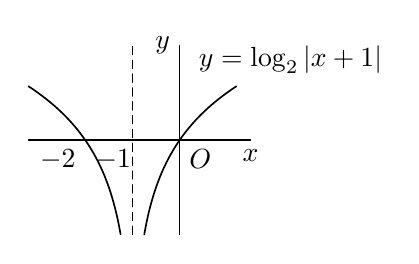
\begin{tikzpicture}[line cap=round,line join=round,scale=0.6]
      \draw[\myaxisarrow] (-3.2,0) -- (1.5,0) node[below] {$x$};
      \draw[\myaxisarrow] (0,-2) -- (0,2) node[left] {$y$};
      \draw[line width=0.6pt,smooth,samples=100] 
        plot[domain=-0.75:1.2](\x,{ln(\x+1)/ln(2)})
        plot[domain=-3.2:-1.25](\x,{ln(-\x-1)/ln(2)});
      \draw[densely dashed] (-1,-2)--(-1,2);
      \draw (0,0) node[anchor=north west] {$O$}
        (-1,0) node[anchor=north east,xshift=3pt] {$-1$} 
        (-2,0) node[anchor=north east] {$-2$}
        (0.2,1.7) node[right] {$y=\log_2 |x+1|$};
    \end{tikzpicture}\end{center}}
    和原图象一起构成 $y=\log_2 |x|$ 的图象, 再整体向左平移 $1$ 个单位长度可得 $y=\log_2 |x+1|$ 的图象, 如右图所示, 在 $(-\infty,-1)$ 上 $\searrow$, 在 $(-1,+\infty)$ 上 $\nearrow$.  
  \endsolution
  
  \lianxi
  \begin{exercise}[s]
    若函数 $y=\log_a x$ ($a>0$, 且 $a\neq1$) 
    的图象如图~\ref{fig-190417-2220}~中第一个图所示,
    则 (1)---(3) 中函数图象正确的是\,?
    \begin{figure}[htb]
    \small
    \centering
    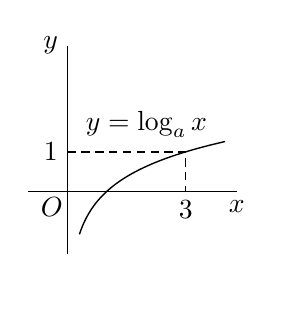
\begin{tikzpicture}[scale=0.5]
      \draw[\myaxisarrow] (-1,0) -- (4.3,0) node[below] {$x$};
      \draw[\myaxisarrow] (0,-1.6) -- (0,3.7) node[left] {$y$};
      \draw[line width=0.5pt,densely dashed]
        (0,1)--(3,1)--(3,0);
      \draw[line width=0.5pt,smooth,samples=100,domain=0.3:4] 
        plot(\x,{ln(\x)/ln(3)});
      \draw (2,1.7) node {$y=\log_a x$};
      \draw (3,0) node[below] {$3$};
      \draw (0,1) node[left] {$1$};
      \draw (-0.4,-0.4) node {$O$};
      \draw (0.5,-2.7) node {};
    \end{tikzpicture}\hskip 0.3cm
    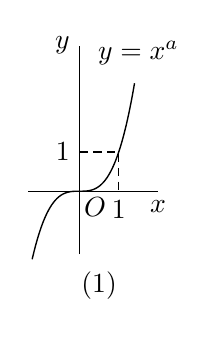
\begin{tikzpicture}[scale=0.5]
      \draw[\myaxisarrow] (-1.3,0) -- (2,0) node[below] {$x$};
      \draw[\myaxisarrow] (0,-1.6) -- (0,3.7) node[left] {$y$};
      \draw[line width=0.5pt,densely dashed]
        (0,1)--(1,1)--(1,0);
      \draw[line width=0.5pt,smooth,samples=100,domain=-1.2:1.4] 
        plot(\x,{(\x)^3});
      \draw (1.5,3.5) node {$y=x^a$};
      \draw (1,0) node[below] {$1$};
      \draw (0,1) node[left] {$1$};
      \draw (0.4,-0.4) node {$O$};
      \draw (0.5,-2.4) node {$(1)$};
    \end{tikzpicture}\hskip 0.3cm
    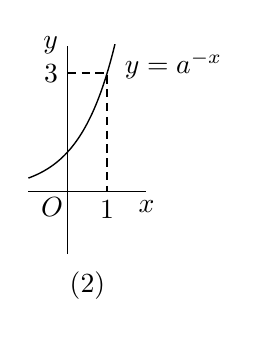
\begin{tikzpicture}[scale=0.5]
      \draw[\myaxisarrow] (-1,0) -- (2,0) node[below] {$x$};
      \draw[\myaxisarrow] (0,-1.6) -- (0,3.7) node[left] {$y$};
      \draw[line width=0.5pt,densely dashed]
        (0,3)--(1,3)--(1,0);
      \draw[line width=0.5pt,smooth,samples=100,domain=-1:1.2] 
        plot(\x,{3^(\x)});
      \draw (1.2,3.2) node[right] {$y=a^{-x}$};
      \draw (1,0) node[below] {$1$};
      \draw (0,3) node[left] {$3$};
      \draw (-0.4,-0.4) node {$O$};
      \draw (0.5,-2.4) node {$(2)$};
    \end{tikzpicture}\hskip 0.3cm
    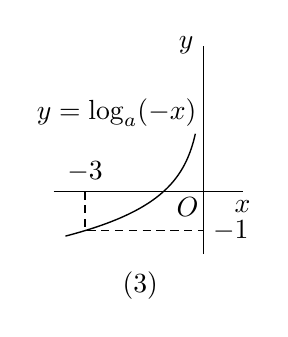
\begin{tikzpicture}[scale=0.5]
      \draw[\myaxisarrow] (-3.8,0) -- (1,0) node[below] {$x$};
      \draw[\myaxisarrow] (0,-1.6) -- (0,3.7) node[left] {$y$};
      \draw[line width=0.5pt,densely dashed]
        (-3,0)--(-3,-1)--(0,-1);
      \draw[line width=0.5pt,smooth,samples=100,domain=-3.5:-0.2] 
        plot(\x,{-ln(-\x)/ln(3)});
      \draw (-2.2,2) node {$y=\log_a(-x)$};
      \draw (-3,0) node[above] {$-3$};
      \draw (0,-1) node[right] {$-1$};
      \draw (-0.4,-0.4) node {$O$};
      \draw (-1.6,-2.4) node {$(3)$};
    \end{tikzpicture}
    \caption{}\label{fig-190417-2220}
    \end{figure}
  \end{exercise}

  \beginsolution
    由 $\log_a 3=1$ 知 $a=3$, 故只有 (1) 中的图象正确.
  \endsolution
  
  \subsubsection{课堂评价}
  \begin{exercise}
    已知函数 $f(x)=\lg x$, 若 $f(ab)=1$, 求 $f(a^2)+f(b^2)=$ 的值.
  \end{exercise}

  \beginsolution
    $\lg(ab)=1$, 则 $f(a^2)+f(b^2)=2\lg(ab)=2$.
  \endsolution
  
  \begin{exercise}
    已知 $a=\log_2 3+\log_2\sqrt3$, $b=\log_2 9-\log_2\sqrt3$, 
    $c=\log_3 2$, 确定 $a$, $b$, $c$ 的大小关系.
  \end{exercise}

  \beginsolution
    $a=\frac32\log_2 3=b>1>c$, 即 $a=b>c$.
    \mymarginpar{比较两个数的大小除了借助中间值 (如 $0$, $1$ 等) 外, 还有
    \[\begin{aligned}
      a-b>0 &\Leftrightarrow a>b;\\
      \frac{a}b>1 &\Leftrightarrow a>b\ (b>0).
      \end{aligned}\]
      通用方法是利用函数的单调性.}
    
    \varexercise 比较 $a=\log_2 3$ 与 $b=\log_3 16$ 的大小.
    
    $\log_2 3<2< \log_3 16$, 即 $a<b$.
    
    \varexercise 比较 $a=\log_2 3$ 与 $b=\log_3 4$ 的大小.
    
    因为 
    \[\frac{a}b= \frac{\ln3}{\ln2}\cdot \frac{\ln3}{2\ln2}
      =\Big(\frac{\ln3}{\sqrt2\ln2}\Big)^2,\]
    且 $2^{\sqrt2}< 2^{1.5}= 2\sqrt2= 2.828\cdots< 3$, 所以 $\frac{\ln3}{\sqrt2\ln2}>1$, 即 $\frac{a}b>1$. 由 $b>0$ 知 $a>b$.
    
    \varexercise 比较 $a=\log_2 3$ 与 $b=\log_3 8$ 的大小.
    
    因为 
    \[\frac{a}b= \frac{\ln3}{\ln2}\cdot \frac{\ln3}{3\ln2}
      =\Big(\frac{\ln3}{\sqrt3\ln2}\Big)^2,\]
    所以需要比较 $3$ 与 $2^{\sqrt3}$ 的大小. 由 $2^8=256>243=3^5$ 知 $2^{1.6}>3$, 故 $2^{\sqrt3}>2^{1.6}>3$, 所以 $\frac{a}b<1$. 由 $b>0$ 知 $a<b$.
  \endsolution
  
  \begin{exercise}
    已知 $f(x)=\log_3 x$, 求 $f\Big(\frac{\sqrt3}3\Big)$ 的值.
  \end{exercise}

  \beginsolution
    $f\Big(\frac{\sqrt3}3\Big)= \log_3 3^{-\frac12}= -\frac12$.
  \endsolution
  
  \begin{exercise}
    求函数 $f(x)=\ln(x^2 -x)$ 的定义域.
  \end{exercise}

  \beginsolution
    $x^2-x>0$, 则 $x\in(-\infty,0)\cup(1,+\infty)$.
  \endsolution
  
  \subsection{课后练习}
  \begin{exercise}
    若函数 $f(x)=\begin{cases}
      x^2+1, & x\leqslant 1,\\
      \lg x, & x>1,
    \end{cases}$ 求 $f\big(f(10)\big)$ 的值.
  \end{exercise}

  \beginsolution
    $f\big(f(10)\big)=f(1)=2$.
  \endsolution
  
  \begin{exercise}
    求函数 $f(x)=1+\log_a (x^2-1)$ 的图象经过的定点.
  \end{exercise}

  \beginsolution
    图象过定点 $(-\sqrt2,1)$ 和 $(\sqrt2,1)$.
  \endsolution
  
  \begin{exercise}
    函数 $y=1+\ln\frac{1+x}{1-x}$ 的图象关于$\underline{\qquad\qquad}$对称.
  \end{exercise}

  \beginsolution
    函数 $y-1$ 为奇函数, 关于原点对称, 所以 $y$ 的图象关于 $(0,1)$ 对称.
  \endsolution
  
  \begin{exercise}
    函数 $f(x)=\frac1{\sqrt{\log_2 x-1}}$ 的定义域为\,?
  \end{exercise}

  \beginsolution
    $\log_2 x-1>0$, 则 $x\in(2,+\infty)$.
  \endsolution
  
  \begin{exercise}
    若 $\log_a\frac{12}{a-1}<1$, 求 $a$ 的取值范围.
  \end{exercise}

  \beginsolution
    由题, $\frac{12}{a-1}>0$, 则 $a>1$, 原不等式化为 $\frac{12}{a-1}<a$, 解得 $a\in(4,+\infty)$.
  \endsolution
  
  \begin{exercise}
    已知函数 $f(x)=|\log_2 x|$, 正实数 $m<n$ 满足 $f(m)=f(n)$. 
    若函数 $f(x)$ 在区间 $[m^2,n]$ 上的最大值为 $2$, 则 $m+n=$\,?
  \end{exercise}

  \beginsolution
    由 $f(x)$ 的图象知 $0<m<1<n$, 
    \mymarginpar{函数 $f(x)=|\log_2 x|$ 的图象:
    \begin{center}
    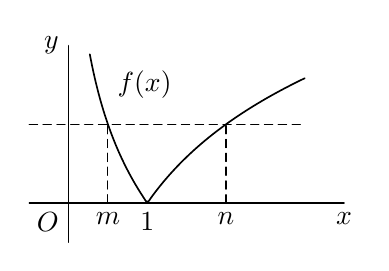
\begin{tikzpicture}[line cap=round,line join=round,scale=1]
      \draw[\myaxisarrow] (-0.5,0) -- (3.5,0) node[below] {$x$};
      \draw[\myaxisarrow] (0,-0.5) -- (0,2) node[left] {$y$};
      \draw[line width=0.6pt,smooth,samples=100] 
        plot[domain=0.27:3](\x,{abs(ln(\x)/ln(2))});
      \draw[densely dashed] (-0.5,1)--(3,1) (0.5,0)--(0.5,1) (2,0)--(2,1);
      \draw (0,0) node[anchor=north east] {$O$}
        (1,0) node[below] {$1$} 
        (0.5,0) node[below] {$m$}
        (2,0) node[below] {$n$}
        (0.5,1.5) node[right] {$f(x)$};
    \end{tikzpicture}\end{center}}
    则 $f(m)=f(n)$ 化为 $-\log_2 m=\log_2 n$, 即 $mn=1$. 由 $m^2<m$ 知 $f(x)$ 在区间 $[m^2,n]$ 上的最大值为 $f(m^2)=2$, 解得 $m=\frac12$. 所以 $n=2$, $m+n=\frac52$.
  \endsolution

  \begin{exercise}
    已知 $2^x =3^y =5^z$, 且 $x$, $y$, $z$ 都是正数, 
    比较 $2x$, $3y$, $5z$ 的大小.
  \end{exercise}
  
  \beginsolution
    设 $2^x=3^y=5^z=k$, 则 $k>1$ 且
    \[2x=\frac{2\ln k}{\ln 2},\quad 3y=\frac{3\ln k}{\ln 3},\quad 5z=\frac{5\ln k}{\ln 5}.\]
    由 $\frac{3}{\ln3}< \frac{2}{\ln2}< \frac{5}{\ln5}$ 和 $\ln k>0$ 知 $3y<2x<5z$.
    
    \varexercise 若 $6^x=7^y=8^z$, 比较 $6x$, $7y$, $8z$ 的大小.
    
    设 $6^x=7^y=8^z=k$, 则
    \[6x=\frac{\ln k}{\ln 6^{1/6}},\quad 7y=\frac{\ln k}{\ln 7^{1/7}},\quad 8z=\frac{\ln k}{\ln 8^{1/8}}.\]
    由 $f(x)=x^{\frac1x}$ 在 $[\mathrm{e},+\infty)$ 上 $\searrow$ 且 $f(x)>1$ 知, 若 $k>1$ 则 $\ln k>0$, $6x<7y<8z$; 若 $0<k<1$ 则 $\ln k<0$, $6x>7y>8z$.
  \endsolution
  
  \begin{exercise}
    如图~\ref{fig-191105-2100}, 点~$A$, $B$ 在函数 $f(x)=\log_2 x+2$ 的图象上, 点~$C$ 在函数 $g(x)=\log_2 x$ 的图象上. 设点~$A$ 的坐标为 $(m,n)$, 若 $\triangle ABC$ 为等边三角形且直线~$BC\parallel y$~轴, 求 $m$ 的值.
  \begin{figure}[htb]
    \small
    \centering
    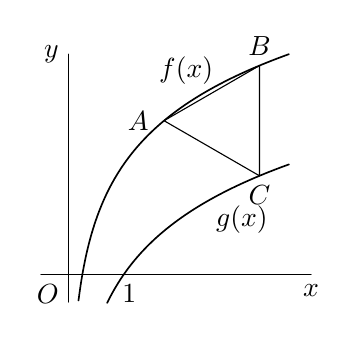
\begin{tikzpicture}[line cap=round,line join=round,scale=0.7]
      \draw[\myaxisarrow] (-0.5,0) -- (4.4,0) node[below] {$x$};
      \draw[\myaxisarrow] (0,-0.5) -- (0,4) node[left] {$y$};
      \draw[line width=0.6pt,smooth,samples=100] 
        plot[domain=0.7:4](\x,{ln(\x)/ln(2)})
        plot[domain=0.18:4](\x,{ln(\x)/ln(2)+2});
      \draw (0,0) node[anchor=north east] {$O$}
        ({sqrt(3)},{ln(sqrt(3))/ln(2)+2}) node[left,xshift=-2pt] {$A$} coordinate (A)
        --++({sqrt(3)},1) node[above] {$B$}
        --++(0,-2) node[below] {$C$} --(A)
        (1,0) node[below,xshift=2pt] {$1$}
        (2.8,3.7) node[left] {$f(x)$}
        (2.5,1) node[right] {$g(x)$};
    \end{tikzpicture}
    \caption{}\label{fig-191105-2100}
  \end{figure}
  \end{exercise}

  \beginsolution
    由 $A(m,n)$ 知 $B(m+\sqrt3,n+1)$, 代入 $f(x)$,
    \[\log_2 m+2=n,\quad \log_2(m+\sqrt3)+2= n+1,\]
    作差得 $\log_2\frac{m+\sqrt3}m=1$, 解得 $m=\sqrt3$.
  \endsolution
  
%%%%%%%%%%%%%%%%%%%%%%%%%%%%%%%%%%%%%%%%%%